% Created by tikzDevice version 0.10.1 on 2016-09-04 20:33:19
% !TEX encoding = UTF-8 Unicode
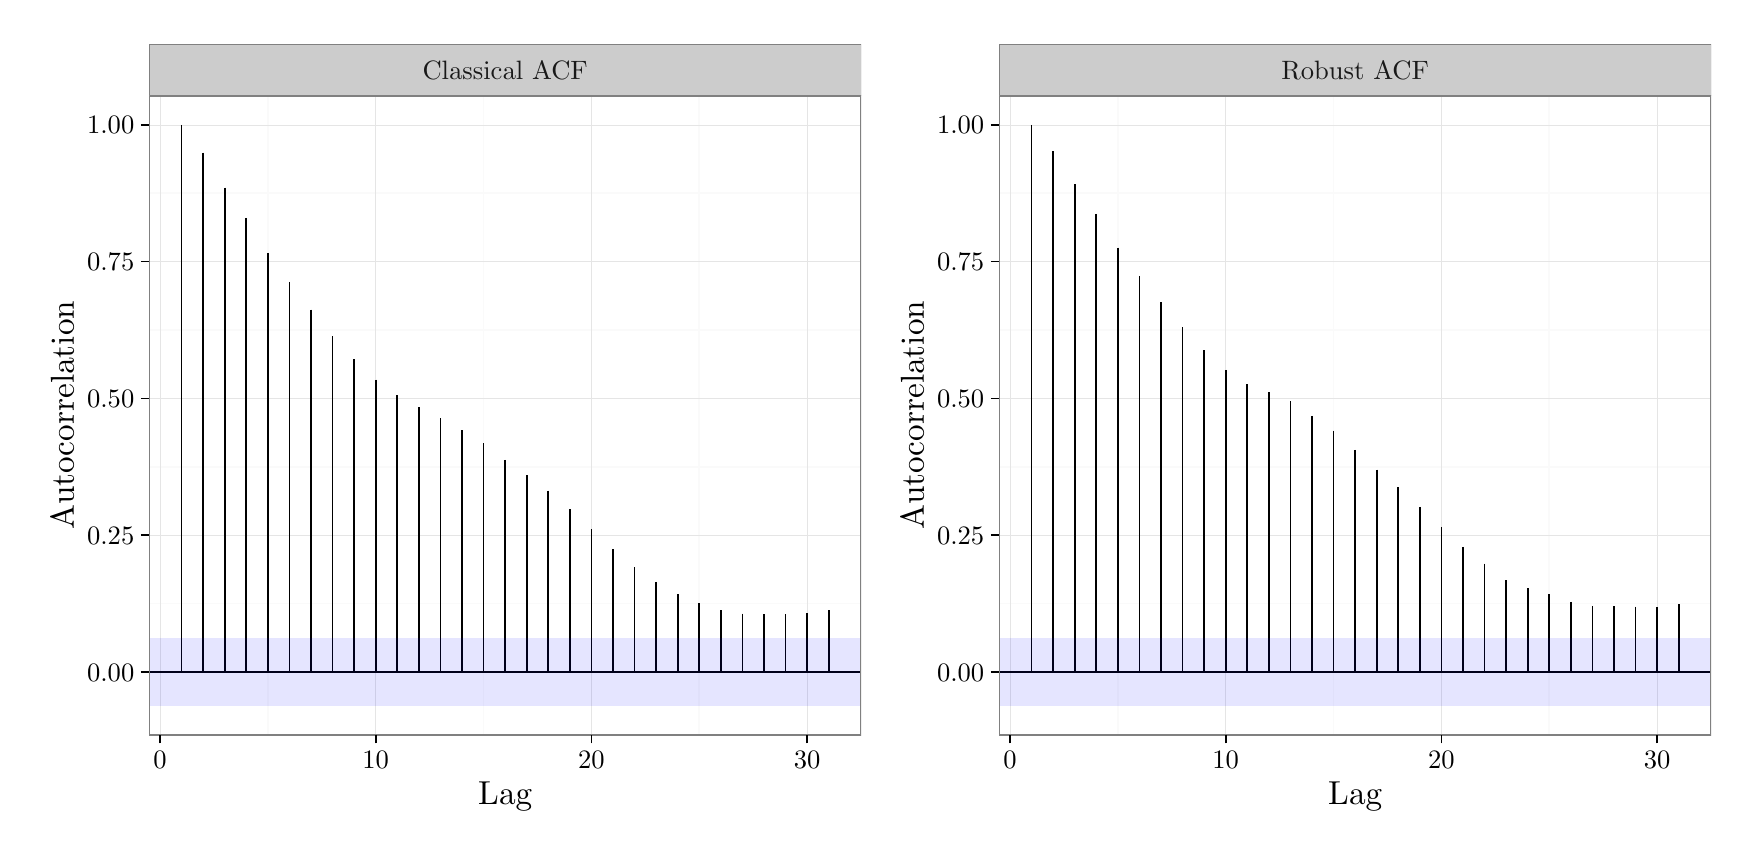
\begin{tikzpicture}[x=1pt,y=1pt]
\definecolor{fillColor}{RGB}{255,255,255}
\path[use as bounding box,fill=fillColor,fill opacity=0.00] (0,0) rectangle (614.29,289.08);
\begin{scope}
\path[clip] (  0.00,  0.00) rectangle (307.15,289.08);
\definecolor{drawColor}{RGB}{255,255,255}
\definecolor{fillColor}{RGB}{255,255,255}

\path[draw=drawColor,line width= 0.6pt,line join=round,line cap=round,fill=fillColor] ( -0.00,  0.00) rectangle (307.15,289.08);
\end{scope}
\begin{scope}
\path[clip] ( 43.93, 33.48) rectangle (301.15,264.47);
\definecolor{fillColor}{RGB}{255,255,255}

\path[fill=fillColor] ( 43.93, 33.48) rectangle (301.15,264.47);
\definecolor{drawColor}{gray}{0.98}

\path[draw=drawColor,line width= 0.6pt,line join=round] ( 43.93, 80.95) --
	(301.15, 80.95);

\path[draw=drawColor,line width= 0.6pt,line join=round] ( 43.93,130.38) --
	(301.15,130.38);

\path[draw=drawColor,line width= 0.6pt,line join=round] ( 43.93,179.82) --
	(301.15,179.82);

\path[draw=drawColor,line width= 0.6pt,line join=round] ( 43.93,229.25) --
	(301.15,229.25);

\path[draw=drawColor,line width= 0.6pt,line join=round] ( 86.80, 33.48) --
	( 86.80,264.47);

\path[draw=drawColor,line width= 0.6pt,line join=round] (164.74, 33.48) --
	(164.74,264.47);

\path[draw=drawColor,line width= 0.6pt,line join=round] (242.69, 33.48) --
	(242.69,264.47);
\definecolor{drawColor}{gray}{0.90}

\path[draw=drawColor,line width= 0.2pt,line join=round] ( 43.93, 56.23) --
	(301.15, 56.23);

\path[draw=drawColor,line width= 0.2pt,line join=round] ( 43.93,105.67) --
	(301.15,105.67);

\path[draw=drawColor,line width= 0.2pt,line join=round] ( 43.93,155.10) --
	(301.15,155.10);

\path[draw=drawColor,line width= 0.2pt,line join=round] ( 43.93,204.53) --
	(301.15,204.53);

\path[draw=drawColor,line width= 0.2pt,line join=round] ( 43.93,253.97) --
	(301.15,253.97);

\path[draw=drawColor,line width= 0.2pt,line join=round] ( 47.82, 33.48) --
	( 47.82,264.47);

\path[draw=drawColor,line width= 0.2pt,line join=round] (125.77, 33.48) --
	(125.77,264.47);

\path[draw=drawColor,line width= 0.2pt,line join=round] (203.72, 33.48) --
	(203.72,264.47);

\path[draw=drawColor,line width= 0.2pt,line join=round] (281.66, 33.48) --
	(281.66,264.47);
\definecolor{drawColor}{RGB}{0,0,0}

\path[draw=drawColor,line width= 0.6pt,line join=round] ( 43.93, 56.23) -- (301.15, 56.23);

\path[draw=drawColor,line width= 0.6pt,line join=round] ( 55.62,253.97) -- ( 55.62, 56.23);

\path[draw=drawColor,line width= 0.6pt,line join=round] ( 63.41,243.96) -- ( 63.41, 56.23);

\path[draw=drawColor,line width= 0.6pt,line join=round] ( 71.21,231.31) -- ( 71.21, 56.23);

\path[draw=drawColor,line width= 0.6pt,line join=round] ( 79.00,220.33) -- ( 79.00, 56.23);

\path[draw=drawColor,line width= 0.6pt,line join=round] ( 86.80,207.74) -- ( 86.80, 56.23);

\path[draw=drawColor,line width= 0.6pt,line join=round] ( 94.59,197.23) -- ( 94.59, 56.23);

\path[draw=drawColor,line width= 0.6pt,line join=round] (102.39,187.17) -- (102.39, 56.23);

\path[draw=drawColor,line width= 0.6pt,line join=round] (110.18,177.62) -- (110.18, 56.23);

\path[draw=drawColor,line width= 0.6pt,line join=round] (117.98,169.19) -- (117.98, 56.23);

\path[draw=drawColor,line width= 0.6pt,line join=round] (125.77,161.86) -- (125.77, 56.23);

\path[draw=drawColor,line width= 0.6pt,line join=round] (133.56,156.25) -- (133.56, 56.23);

\path[draw=drawColor,line width= 0.6pt,line join=round] (141.36,151.97) -- (141.36, 56.23);

\path[draw=drawColor,line width= 0.6pt,line join=round] (149.15,147.89) -- (149.15, 56.23);

\path[draw=drawColor,line width= 0.6pt,line join=round] (156.95,143.52) -- (156.95, 56.23);

\path[draw=drawColor,line width= 0.6pt,line join=round] (164.74,138.85) -- (164.74, 56.23);

\path[draw=drawColor,line width= 0.6pt,line join=round] (172.54,132.90) -- (172.54, 56.23);

\path[draw=drawColor,line width= 0.6pt,line join=round] (180.33,127.34) -- (180.33, 56.23);

\path[draw=drawColor,line width= 0.6pt,line join=round] (188.13,121.82) -- (188.13, 56.23);

\path[draw=drawColor,line width= 0.6pt,line join=round] (195.92,115.02) -- (195.92, 56.23);

\path[draw=drawColor,line width= 0.6pt,line join=round] (203.72,107.83) -- (203.72, 56.23);

\path[draw=drawColor,line width= 0.6pt,line join=round] (211.51,100.67) -- (211.51, 56.23);

\path[draw=drawColor,line width= 0.6pt,line join=round] (219.30, 94.17) -- (219.30, 56.23);

\path[draw=drawColor,line width= 0.6pt,line join=round] (227.10, 88.81) -- (227.10, 56.23);

\path[draw=drawColor,line width= 0.6pt,line join=round] (234.89, 84.42) -- (234.89, 56.23);

\path[draw=drawColor,line width= 0.6pt,line join=round] (242.69, 81.04) -- (242.69, 56.23);

\path[draw=drawColor,line width= 0.6pt,line join=round] (250.48, 78.63) -- (250.48, 56.23);

\path[draw=drawColor,line width= 0.6pt,line join=round] (258.28, 77.34) -- (258.28, 56.23);

\path[draw=drawColor,line width= 0.6pt,line join=round] (266.07, 77.16) -- (266.07, 56.23);

\path[draw=drawColor,line width= 0.6pt,line join=round] (273.87, 77.09) -- (273.87, 56.23);

\path[draw=drawColor,line width= 0.6pt,line join=round] (281.66, 77.42) -- (281.66, 56.23);

\path[draw=drawColor,line width= 0.6pt,line join=round] (289.46, 78.62) -- (289.46, 56.23);
\definecolor{fillColor}{RGB}{0,0,255}

\path[fill=fillColor,fill opacity=0.10] ( 43.93, 43.98) rectangle (301.15, 68.49);
\definecolor{drawColor}{gray}{0.50}

\path[draw=drawColor,line width= 0.6pt,line join=round,line cap=round] ( 43.93, 33.48) rectangle (301.15,264.47);
\end{scope}
\begin{scope}
\path[clip] ( 43.93,264.47) rectangle (301.15,283.08);
\definecolor{drawColor}{gray}{0.50}
\definecolor{fillColor}{gray}{0.80}

\path[draw=drawColor,line width= 0.2pt,line join=round,line cap=round,fill=fillColor] ( 43.93,264.47) rectangle (301.15,283.08);
\definecolor{drawColor}{gray}{0.10}

\node[text=drawColor,anchor=base,inner sep=0pt, outer sep=0pt, scale=  0.96] at (172.54,270.47) {Classical ACF};
\end{scope}
\begin{scope}
\path[clip] (  0.00,  0.00) rectangle (614.29,289.08);
\definecolor{drawColor}{RGB}{0,0,0}

\node[text=drawColor,anchor=base east,inner sep=0pt, outer sep=0pt, scale=  0.96] at ( 38.53, 52.93) {0.00};

\node[text=drawColor,anchor=base east,inner sep=0pt, outer sep=0pt, scale=  0.96] at ( 38.53,102.36) {0.25};

\node[text=drawColor,anchor=base east,inner sep=0pt, outer sep=0pt, scale=  0.96] at ( 38.53,151.79) {0.50};

\node[text=drawColor,anchor=base east,inner sep=0pt, outer sep=0pt, scale=  0.96] at ( 38.53,201.23) {0.75};

\node[text=drawColor,anchor=base east,inner sep=0pt, outer sep=0pt, scale=  0.96] at ( 38.53,250.66) {1.00};
\end{scope}
\begin{scope}
\path[clip] (  0.00,  0.00) rectangle (614.29,289.08);
\definecolor{drawColor}{RGB}{0,0,0}

\path[draw=drawColor,line width= 0.6pt,line join=round] ( 40.93, 56.23) --
	( 43.93, 56.23);

\path[draw=drawColor,line width= 0.6pt,line join=round] ( 40.93,105.67) --
	( 43.93,105.67);

\path[draw=drawColor,line width= 0.6pt,line join=round] ( 40.93,155.10) --
	( 43.93,155.10);

\path[draw=drawColor,line width= 0.6pt,line join=round] ( 40.93,204.53) --
	( 43.93,204.53);

\path[draw=drawColor,line width= 0.6pt,line join=round] ( 40.93,253.97) --
	( 43.93,253.97);
\end{scope}
\begin{scope}
\path[clip] (  0.00,  0.00) rectangle (614.29,289.08);
\definecolor{drawColor}{RGB}{0,0,0}

\path[draw=drawColor,line width= 0.6pt,line join=round] ( 47.82, 30.48) --
	( 47.82, 33.48);

\path[draw=drawColor,line width= 0.6pt,line join=round] (125.77, 30.48) --
	(125.77, 33.48);

\path[draw=drawColor,line width= 0.6pt,line join=round] (203.72, 30.48) --
	(203.72, 33.48);

\path[draw=drawColor,line width= 0.6pt,line join=round] (281.66, 30.48) --
	(281.66, 33.48);
\end{scope}
\begin{scope}
\path[clip] (  0.00,  0.00) rectangle (614.29,289.08);
\definecolor{drawColor}{RGB}{0,0,0}

\node[text=drawColor,anchor=base,inner sep=0pt, outer sep=0pt, scale=  0.96] at ( 47.82, 21.46) {0};

\node[text=drawColor,anchor=base,inner sep=0pt, outer sep=0pt, scale=  0.96] at (125.77, 21.46) {10};

\node[text=drawColor,anchor=base,inner sep=0pt, outer sep=0pt, scale=  0.96] at (203.72, 21.46) {20};

\node[text=drawColor,anchor=base,inner sep=0pt, outer sep=0pt, scale=  0.96] at (281.66, 21.46) {30};
\end{scope}
\begin{scope}
\path[clip] (  0.00,  0.00) rectangle (614.29,289.08);
\definecolor{drawColor}{RGB}{0,0,0}

\node[text=drawColor,anchor=base,inner sep=0pt, outer sep=0pt, scale=  1.20] at (172.54,  8.40) {Lag};
\end{scope}
\begin{scope}
\path[clip] (  0.00,  0.00) rectangle (614.29,289.08);
\definecolor{drawColor}{RGB}{0,0,0}

\node[text=drawColor,rotate= 90.00,anchor=base,inner sep=0pt, outer sep=0pt, scale=  1.20] at ( 16.66,148.97) {Autocorrelation};
\end{scope}
\begin{scope}
\path[clip] (307.15,  0.00) rectangle (614.29,289.08);
\definecolor{drawColor}{RGB}{255,255,255}
\definecolor{fillColor}{RGB}{255,255,255}

\path[draw=drawColor,line width= 0.6pt,line join=round,line cap=round,fill=fillColor] (307.15,  0.00) rectangle (614.30,289.08);
\end{scope}
\begin{scope}
\path[clip] (351.07, 33.48) rectangle (608.29,264.47);
\definecolor{fillColor}{RGB}{255,255,255}

\path[fill=fillColor] (351.07, 33.48) rectangle (608.29,264.47);
\definecolor{drawColor}{gray}{0.98}

\path[draw=drawColor,line width= 0.6pt,line join=round] (351.07, 80.95) --
	(608.29, 80.95);

\path[draw=drawColor,line width= 0.6pt,line join=round] (351.07,130.38) --
	(608.29,130.38);

\path[draw=drawColor,line width= 0.6pt,line join=round] (351.07,179.82) --
	(608.29,179.82);

\path[draw=drawColor,line width= 0.6pt,line join=round] (351.07,229.25) --
	(608.29,229.25);

\path[draw=drawColor,line width= 0.6pt,line join=round] (393.94, 33.48) --
	(393.94,264.47);

\path[draw=drawColor,line width= 0.6pt,line join=round] (471.89, 33.48) --
	(471.89,264.47);

\path[draw=drawColor,line width= 0.6pt,line join=round] (549.84, 33.48) --
	(549.84,264.47);
\definecolor{drawColor}{gray}{0.90}

\path[draw=drawColor,line width= 0.2pt,line join=round] (351.07, 56.23) --
	(608.29, 56.23);

\path[draw=drawColor,line width= 0.2pt,line join=round] (351.07,105.67) --
	(608.29,105.67);

\path[draw=drawColor,line width= 0.2pt,line join=round] (351.07,155.10) --
	(608.29,155.10);

\path[draw=drawColor,line width= 0.2pt,line join=round] (351.07,204.53) --
	(608.29,204.53);

\path[draw=drawColor,line width= 0.2pt,line join=round] (351.07,253.97) --
	(608.29,253.97);

\path[draw=drawColor,line width= 0.2pt,line join=round] (354.97, 33.48) --
	(354.97,264.47);

\path[draw=drawColor,line width= 0.2pt,line join=round] (432.92, 33.48) --
	(432.92,264.47);

\path[draw=drawColor,line width= 0.2pt,line join=round] (510.86, 33.48) --
	(510.86,264.47);

\path[draw=drawColor,line width= 0.2pt,line join=round] (588.81, 33.48) --
	(588.81,264.47);
\definecolor{drawColor}{RGB}{0,0,0}

\path[draw=drawColor,line width= 0.6pt,line join=round] (351.07, 56.23) -- (608.29, 56.23);

\path[draw=drawColor,line width= 0.6pt,line join=round] (362.77,253.97) -- (362.77, 56.23);

\path[draw=drawColor,line width= 0.6pt,line join=round] (370.56,244.50) -- (370.56, 56.23);

\path[draw=drawColor,line width= 0.6pt,line join=round] (378.36,232.47) -- (378.36, 56.23);

\path[draw=drawColor,line width= 0.6pt,line join=round] (386.15,221.80) -- (386.15, 56.23);

\path[draw=drawColor,line width= 0.6pt,line join=round] (393.94,209.60) -- (393.94, 56.23);

\path[draw=drawColor,line width= 0.6pt,line join=round] (401.74,199.36) -- (401.74, 56.23);

\path[draw=drawColor,line width= 0.6pt,line join=round] (409.53,189.93) -- (409.53, 56.23);

\path[draw=drawColor,line width= 0.6pt,line join=round] (417.33,180.76) -- (417.33, 56.23);

\path[draw=drawColor,line width= 0.6pt,line join=round] (425.12,172.47) -- (425.12, 56.23);

\path[draw=drawColor,line width= 0.6pt,line join=round] (432.92,165.41) -- (432.92, 56.23);

\path[draw=drawColor,line width= 0.6pt,line join=round] (440.71,160.30) -- (440.71, 56.23);

\path[draw=drawColor,line width= 0.6pt,line join=round] (448.51,157.37) -- (448.51, 56.23);

\path[draw=drawColor,line width= 0.6pt,line join=round] (456.30,154.00) -- (456.30, 56.23);

\path[draw=drawColor,line width= 0.6pt,line join=round] (464.10,148.80) -- (464.10, 56.23);

\path[draw=drawColor,line width= 0.6pt,line join=round] (471.89,143.44) -- (471.89, 56.23);

\path[draw=drawColor,line width= 0.6pt,line join=round] (479.68,136.53) -- (479.68, 56.23);

\path[draw=drawColor,line width= 0.6pt,line join=round] (487.48,129.37) -- (487.48, 56.23);

\path[draw=drawColor,line width= 0.6pt,line join=round] (495.27,123.07) -- (495.27, 56.23);

\path[draw=drawColor,line width= 0.6pt,line join=round] (503.07,115.89) -- (503.07, 56.23);

\path[draw=drawColor,line width= 0.6pt,line join=round] (510.86,108.73) -- (510.86, 56.23);

\path[draw=drawColor,line width= 0.6pt,line join=round] (518.66,101.46) -- (518.66, 56.23);

\path[draw=drawColor,line width= 0.6pt,line join=round] (526.45, 95.44) -- (526.45, 56.23);

\path[draw=drawColor,line width= 0.6pt,line join=round] (534.25, 89.41) -- (534.25, 56.23);

\path[draw=drawColor,line width= 0.6pt,line join=round] (542.04, 86.55) -- (542.04, 56.23);

\path[draw=drawColor,line width= 0.6pt,line join=round] (549.84, 84.26) -- (549.84, 56.23);

\path[draw=drawColor,line width= 0.6pt,line join=round] (557.63, 81.55) -- (557.63, 56.23);

\path[draw=drawColor,line width= 0.6pt,line join=round] (565.42, 80.18) -- (565.42, 56.23);

\path[draw=drawColor,line width= 0.6pt,line join=round] (573.22, 80.08) -- (573.22, 56.23);

\path[draw=drawColor,line width= 0.6pt,line join=round] (581.01, 79.84) -- (581.01, 56.23);

\path[draw=drawColor,line width= 0.6pt,line join=round] (588.81, 79.64) -- (588.81, 56.23);

\path[draw=drawColor,line width= 0.6pt,line join=round] (596.60, 80.70) -- (596.60, 56.23);
\definecolor{fillColor}{RGB}{0,0,255}

\path[fill=fillColor,fill opacity=0.10] (351.07, 43.98) rectangle (608.29, 68.49);
\definecolor{drawColor}{gray}{0.50}

\path[draw=drawColor,line width= 0.6pt,line join=round,line cap=round] (351.07, 33.48) rectangle (608.29,264.47);
\end{scope}
\begin{scope}
\path[clip] (351.07,264.47) rectangle (608.29,283.08);
\definecolor{drawColor}{gray}{0.50}
\definecolor{fillColor}{gray}{0.80}

\path[draw=drawColor,line width= 0.2pt,line join=round,line cap=round,fill=fillColor] (351.07,264.47) rectangle (608.29,283.08);
\definecolor{drawColor}{gray}{0.10}

\node[text=drawColor,anchor=base,inner sep=0pt, outer sep=0pt, scale=  0.96] at (479.68,270.47) {Robust ACF};
\end{scope}
\begin{scope}
\path[clip] (  0.00,  0.00) rectangle (614.29,289.08);
\definecolor{drawColor}{RGB}{0,0,0}

\node[text=drawColor,anchor=base east,inner sep=0pt, outer sep=0pt, scale=  0.96] at (345.67, 52.93) {0.00};

\node[text=drawColor,anchor=base east,inner sep=0pt, outer sep=0pt, scale=  0.96] at (345.67,102.36) {0.25};

\node[text=drawColor,anchor=base east,inner sep=0pt, outer sep=0pt, scale=  0.96] at (345.67,151.79) {0.50};

\node[text=drawColor,anchor=base east,inner sep=0pt, outer sep=0pt, scale=  0.96] at (345.67,201.23) {0.75};

\node[text=drawColor,anchor=base east,inner sep=0pt, outer sep=0pt, scale=  0.96] at (345.67,250.66) {1.00};
\end{scope}
\begin{scope}
\path[clip] (  0.00,  0.00) rectangle (614.29,289.08);
\definecolor{drawColor}{RGB}{0,0,0}

\path[draw=drawColor,line width= 0.6pt,line join=round] (348.07, 56.23) --
	(351.07, 56.23);

\path[draw=drawColor,line width= 0.6pt,line join=round] (348.07,105.67) --
	(351.07,105.67);

\path[draw=drawColor,line width= 0.6pt,line join=round] (348.07,155.10) --
	(351.07,155.10);

\path[draw=drawColor,line width= 0.6pt,line join=round] (348.07,204.53) --
	(351.07,204.53);

\path[draw=drawColor,line width= 0.6pt,line join=round] (348.07,253.97) --
	(351.07,253.97);
\end{scope}
\begin{scope}
\path[clip] (  0.00,  0.00) rectangle (614.29,289.08);
\definecolor{drawColor}{RGB}{0,0,0}

\path[draw=drawColor,line width= 0.6pt,line join=round] (354.97, 30.48) --
	(354.97, 33.48);

\path[draw=drawColor,line width= 0.6pt,line join=round] (432.92, 30.48) --
	(432.92, 33.48);

\path[draw=drawColor,line width= 0.6pt,line join=round] (510.86, 30.48) --
	(510.86, 33.48);

\path[draw=drawColor,line width= 0.6pt,line join=round] (588.81, 30.48) --
	(588.81, 33.48);
\end{scope}
\begin{scope}
\path[clip] (  0.00,  0.00) rectangle (614.29,289.08);
\definecolor{drawColor}{RGB}{0,0,0}

\node[text=drawColor,anchor=base,inner sep=0pt, outer sep=0pt, scale=  0.96] at (354.97, 21.46) {0};

\node[text=drawColor,anchor=base,inner sep=0pt, outer sep=0pt, scale=  0.96] at (432.92, 21.46) {10};

\node[text=drawColor,anchor=base,inner sep=0pt, outer sep=0pt, scale=  0.96] at (510.86, 21.46) {20};

\node[text=drawColor,anchor=base,inner sep=0pt, outer sep=0pt, scale=  0.96] at (588.81, 21.46) {30};
\end{scope}
\begin{scope}
\path[clip] (  0.00,  0.00) rectangle (614.29,289.08);
\definecolor{drawColor}{RGB}{0,0,0}

\node[text=drawColor,anchor=base,inner sep=0pt, outer sep=0pt, scale=  1.20] at (479.68,  8.40) {Lag};
\end{scope}
\begin{scope}
\path[clip] (  0.00,  0.00) rectangle (614.29,289.08);
\definecolor{drawColor}{RGB}{0,0,0}

\node[text=drawColor,rotate= 90.00,anchor=base,inner sep=0pt, outer sep=0pt, scale=  1.20] at (323.81,148.97) {Autocorrelation};
\end{scope}
\end{tikzpicture}
